\chapter{Credit Mining System Design}
\label{chp:design}

% section overview, main components. Libtorrent as dependency. 
The goal in this thesis is to implement and evaluate a system where it can be used to both invest credit and improve swarm performance. In this thesis, we introduce ``Credit mining system'', an automatic investment framework on swarm with multidimensional gain. With credit mining system, locally, a user can gain credit with internally limited bandwidth allocation without any intervention needed. The credit can be in many forms such as share ratio (upload-to-download ratio), uploaded amount, effort based credit, and many other. From higher perspective, credit mining system will help a swarm to keep alive by providing integral pieces to the peer who need it. Although credit mining system will be implemented in Tribler system, it is possible to apply this feature to any file-sharing system.

Firstly, the dependencies of credit mining system which is \textit{libtorrent}'s s\textit{hare mode} will be elaborated. \texttt{Share mode} is a module which can be activated as an intent to helping a swarm instead of normal content downloading. This module will be explained in detail in section \ref{section:sharemode}. The rest of the section \ref{section:libtorrent} explain other relevant, yet important module that credit mining system can exploit. Afterwards, the design of credit mining system is presented. This system consists of several subroutines which will be explained afterwards in section \ref{section:cmcomponents}. 

\section{Libtorrent}
\label{section:libtorrent}
With \bt~is just a collection of specification, it free to be implemented with any languages. One of most popular implementation is \textit{libtorrent}. \textit{Libtorrent} is written in \texttt{C++} and adopt open-source policy. \textit{Libtorrent} also has \texttt{python} binding which the same language as Tribler implementation. \textit{Libtorrent} started in 2003 by Arvid Norberg and it implemented most of the \bt~specification. Most of the crucial specification such as DHT, IPv6 tracker, PEX, magnet link, multi-tracker, webseed, and many others has been implemented. That is why \textit{libtorrent} is widely used by many torrent client such as Deluge, qBittorrent, Free download managers, and many others.

In this section, we will elaborate some of the \textit{libtorrent} feature that used in credit mining system and within our scope. How priority is managed within \textit{libtorrent} will be explained. After that, \textit{share mode} as the core function we needed is described in detail. The relation to credit mining system with it will be explained to both of them. In the last part, we will focus on the several peer discovery techniques. With the trackless \bt~evolved in early 2008 by DHT protocol \cite{2008:dht:loewenstern}, monitoring trackers may result in inaccurate result. Moreover, the credit mining mechanism heavily rely on real-time data which can not be obtained from querying the community pages. The data can be acquired both directly and indirectly by crawling peers in the swarm.

\subsection{Priority Management}
Determining which part of the file that needed to be downloaded is central component in \bt~implementation. By default, \textit{libtorrent} will look for rarest piece available in the swarm. However, it is possible to change this behavior. \textit{Libtorrent} provides an API with high granularity. Within a \textit{libtorrent} session, a swarm may have different priority compared with other swarm. Higher priority means higher chance to get unchoked. It is done by enlarging peer's bandwidth who has that swarm. In this way, \textit{libtorrent} can always prioritize those peers, therefore, the particular swarm. 

Going deeper into \textit{libtorrent} API, it is also possible to prioritize a particular files or pieces in a swarm as well. It is common to have multiple files assigned in a swarm. A file consists of many pieces. However, one piece may represent one or more file. In a swarm perspective, length of the piece is always same, except the last one. By prioritizing files, \textit{libtorrent} assigned all pieces correlated with that file. Assigning priority to a piece will affect how that piece will be chosen for downloading. By default, \textit{libtorrent} sort the piece by its availability. Therefore, it downloads the rarest piece first before anything else. The piece and file priority can be overridden by calling the API. There are 8 level of priority, with level 0 means never be downloaded. The levels are : 

\begin{enumerate}[topsep=1pt,itemsep=0ex,partopsep=0pt,parsep=2pt]
	\itemsep0em 
	\item[0.] piece is not downloaded at all.
	\item normal priority. How \textit{libtorrent} download it is depending on the piece availability.
	\item higher than normal priority. \textit{Libtorrent} prefer this piece instead of other piece which has same availability
	\item in partial piece mode, picker will prefer to pick this priority on top of other priority
	\item in partial piece mode with the same availability, picker will pick this piece instead of \textit{3)}
	\item this priority is the same as \textit{4)}
	\item this piece is likely to be picked as long as the availability is more than 1
	\item maximum priority. Picker will not consider availability and always prioritize this piece.
\end{enumerate}

Using the mentioned API, credit mining system independently prioritize part of the swarm with various conditions. As will be shown in Section \ref{section:optimization}, the system always prioritize the user downloading activity rather than its mining activity. In other condition, credit mining will trigger the idle mining activity and do an initial download part to measure the swarm. This feature shown later in Chapter \ref{chapter:prospection}. 
%Unchoke round. Bandwidth control.

\subsection{Share Mode}
\label{section:sharemode}
One of the crucial feature used in this work is \textit{share mode} \footnote{Core code of share mode can be found in \url{https://github.com/arvidn/libtorrent/blob/master/src/torrent.cpp\#L9586-L9727}}. Initial work performed by \citeauthor{2015:creditmining:capota} also used this feature\cite{2015:creditmining:capota}. By enabling share mode, it means that one is not interested in downloading the file, but gaining higher share ratio. It is done by download as little as possible and upload as much as possible. Share mode only download a torrent where it has sufficient capacity. A torrent downloaded in share mode may never finish as \textit{libtorrent} only download piece of a torrent which satisfied the share mode requirements. Share mode can be enabled per torrent basis.

Share mode algorithm works heuristically as it estimates the rarest piece available in the swarm based on participated peers. First, it tries to find whether there is a piece which nobody has (line \ref{alg:l_lts:missingp}). Note that in line \ref{alg:l_lts:disconnectpeers}, libtorrent disconnect some of the seeder because we need to connect to the leecher later. This case is considered if there are too many seeder in our connection pool. Next, the number of missing pieces is decreased linearly with the number of seeder. This is based on assumption that both of us and other seeder can upload at least one piece each (line \ref{alg:l_lts:reducemissing}). To keep the performance, downloading piece activity is stacked until more than 5\% of the number to be downloaded (line \ref{alg:l_lts:retdling}). To determine rarest piece, libtorrent count the number of peer that has that piece. The number of peer on the rarest piece is termed \textit{rarity}. Share mode ensure that we only download the rarest piece available in the network (line \ref{alg:l_lts:rarepc}). We end the prematurely routine if there are more number of piece to download compared to uploaded (line \ref{alg:l_lts:retdlenough}) or there are not enough peer to upload the rarest piece (line \ref{alg:l_lts:rareunable}). Both condition will prevent us to get positive share ratio. Finally, it will download randomly the rarest pieces if there are more than one option (line \ref{alg:l_lts:dlrare}). The algorithm presented in algorithm \ref{alg:ltsharemode}. 

\begin{algorithm}[h!]
	\caption{Libtorrent share mode algorithm}
	\label{alg:ltsharemode}
	\begin{algorithmic}[1]
		\Require{$T$ as share mode target}
		\Statex
		\State{$missing\_piece = 0$}
		\ForAll{$p \in connected\_peers$}
		\If{$p$ is a $leecher$ $and$ $p$ is not in share\_mode}	
		\State{$missing\_pieces$} += {$total\_pieces - pieces(p)$} \label{alg:l_lts:missingp}
		\EndIf	
		\EndFor
		\If{$|connected\_seeders|$ in $connected\_peer$ $>$ $90\%$}	
		\State disconnect excess seeder \label{alg:l_lts:disconnectpeers}
		\EndIf
		\State{$missing\_pieces$} -= {$2 \times |connected\_seeders|$}	\label{alg:l_lts:reducemissing}	
		\If{$missing\_pieces \leq 0$}
		\State \Return
		\EndIf
		\If{$num\_downloaded \times T > uploaded$} \label{alg:l_lts:retdlenough}
		\State \Return
		\EndIf
		\If{$downloading > 5\% \times num\_downloaded$} \label{alg:l_lts:retdling}
		\State \Return
		\EndIf
		\ForAll{$pc \in pieces()$}
		\If{$pc$ not in $collected\_piece$ $and$ $peer\_count(pc) \leq rarest\_rarity$ }	\label{alg:l_lts:rarepc}
		\State{$rarest\_rarity$} = {$peer\_count(pc)$} 
		\State{$rare\_piece$.push($pc$)}
		\EndIf	
		\EndFor
		\If{$|connected\_peers| - rarest\_rarity < T$} \label{alg:l_lts:rareunable}
		\State \Return
		\EndIf
		\State download {$random(rare\_piece)$} \label{alg:l_lts:dlrare}
	\end{algorithmic}
\end{algorithm}

There are several limitations on this feature as we observed. First, it only has single parameter which determine the desired target of share ratio. This limits the exploration and full use of share mode feature. Another issues are storage and network inefficiency. If enabled, share mode works by downloading popular piece of a particular torrent. This means few downloaded pieces could take a large storage. Share mode also did not check whether a swarm is efficient enough to perform this operation. It only tries to find popular pieces regardless of the swarm condition. It is highly possible that if a swarm is in poor capacity, the uploading rate is very low. The bandwidth used to check torrent pieces regularly is wasted and the ``investment'' will not go well. The biggest limitation of share mode is the probability of getting bottleneck because of its strict policy. In early stage of joining a swarm, share mode downloaded 1 piece at a time. This can result slower decision making and the rarity of pieces changed. 

Bottleneck can happen in the early time of share mode. The combination of line \ref{alg:l_lts:retdlenough} and \ref{alg:l_lts:retdling} will hold downloading any piece if the uploaded amount is not enough based on the piece we have. Let say we already which piece to download from line \ref{alg:l_lts:dlrare}. In the next round, this piece is not rare anymore. Therefore, we cannot upload this piece.  \todo{expand}
% peer discovery DHT, PEX, LSD
\subsection{Peer Discovery}
One of the integral part in \bt~protocol is peer discovery. With numerous known peers, the algorithm will have more option on which peer to unchoke. State of the swarm itself often represented by the peer belong to that swarm. It is relatively costly just to discover new peers if there are a lot of swarms monitored. \citeauthor{2012:milliontorrent:arvid} shows an example how costly the \textit{announce} request accompanied by \textit{response} payload can be in seeding a lot of torrents. Seeding 1 million torrents with announce once per every hour, which is half of the default interval, need 130 kB/s upload and 75 kB/s download bandwidth constantly \cite{2012:milliontorrent:arvid}. This value is significant for most of common Internet connection.

In \bt, there are four methods to discover new or update peer. Those are using centralized trackers, distributed hash table (DHT), peer exchange (PEX), and local service discovery (LSD). The methods will be described below. To be able fully trackerless, \textit{magnet link} extension is needed in every peer \cite{2008:magnet:hazel}. By magnet link, user can join a swarm and complete the download without using \texttt{.torrent} as its initial data. 

\subsubsection{Tracker Peer Announce}
In original design of \bt, it uses tracker to allow peer discover each other \cite{2003:bittorrent:cohen}. Tracker tends to use random and limited list of peers. Peer contact tracker periodically to expand their peer dictionary. This act of requesting peer to tracker is called \textit{announce}.	Usually, most tracker has a policy about recommended interval when to recontact for getting new peers. Violate this policy can result a particular peer blocked.	

\subsubsection{Distributed Hash Table (DHT)}
Originally, peer needs to contact tracker to fetch new peer address and file information. This makes \bt~very dependent on centralized system which vulnerable to single point of failure. In 2008, Distributed Hash Table (DHT) was proposed \cite{2008:dht:loewenstern}. Towards a ``trackerless'' \bt~system, DHT allows each peer to become a tracker. DHT stores peer contact information with defined key-space as ``node ID''. Each peer stored other peer's node ID and its address in their own routing table. A ``distance'' is measured on two node ID to define how close those two. ``Distance'' also can be measured between infohash of a torrent and node ID.

To enrich its peer dictionary, a node can compare a torrent's infohash and node ID in its routing table. If the distance under the threshold, it contacts that node to ask the information of the swarm, which includes the peer list. If contacted node do not know this torrent, it will respond with another node in its table which closest to the provided infohash. 
%\todo{expand_:DHT performance?}

\subsubsection{Peer Exchange (PEX)}
To increase the chance of getting higher downloading speed, having up to date peer is desired. This can be achieved by contacting tracker or using DHT. Reducing the interval of contacting tracker can result in getting a number of updated peer sooner, however, it will put a burden on the tracker itself. Peer Exchange (PEX )\cite{2015:PEX:the8472} is proposed to tackle this problem. PEX used list of peers that bootstrapped from another mechanism. This mechanism allows contacting known peer directly to get and give up-to-date information on swarm. Theoretically, it can keep this swarm together if trackers are down. Specification mentioned in \cite{2015:PEX:the8472} stated a restriction such as number of request per minute and number of peer added or removed in a PEX message.

\subsubsection{Local Service Directory (LSD)}
To increase the performance when downloading from a swarm, it is preferable to get the file from local network if available. Local service directory (LSD) permit this by discover peers that are in the same local network. The transfer rate is much higher compared to other type of peers. In short, LSD uses multicast-like mechanism which broadcast infohash of a torrent.


\section{Credit Mining Architecture}
\label{section:cmcomponents}

Credit mining system is intended to do its task automatically with minimal user intervention. The way this system designed is to align supply and demand of chosen swarm. Short term advantage of this approach is to gain credit by minimal download and maximize upload. In the long term, this potentially increase overall performance of other user as well.

The system can be implemented beside any torrent client. In Figure \ref{fig:cmcomponents}, it shown the compulsory elements and the relation between \textit{credit mining system} and \textit{torrent client}. Currently, we assume that every torrent client also track how much data a user has been downloaded and uploaded. We called this tracking history as \textit{credit storage} or \textit{bank}. Naturally, any torrent client must have \textit{downloading module} as well. Other dependency are te \textit{libtorrent} library. Credit mining system will use some of the \textit{libtorrent}-specific function. This function is not part of the \bt~Enhancement Protocol (BEP) which define the standard of \bt~protocol that need to be implemented. Other required feature is the ability of discovering peer by all method (DHT, PEX, LSD, etc). In some cases, peer discovery function is disabled for security reasons. While disabling one should not affect credit mining system, it will reduce the prediction and overall performance.

Credit mining system consists of several elements. First is the \textit{credit mining manager}. The \textit{manager} receives the \textit{settings} from user in the initial phase. To control mining process, user can only interact with value at \textit{settings} elements. User also limited to only add and remove \textit{mining source}. Each of the source will be assigned with a \textit{miner} depend on the type of the source. Miner also has sub-elements as part of the system. In-depth explanation of mining source and miners will be discussed in Section \ref{section:msource}. We introduce the \textit{predownload} mechanism as a way to evaluate a source early. This mechanism is launched by the manager instead of miner as it only happen during \textit{early propecting stage}. Predownload mechanism and prospecting methodology in general will be discussed in Chapter \ref{chapter:prospection}.

\begin{figure}[ht]
	\centering
	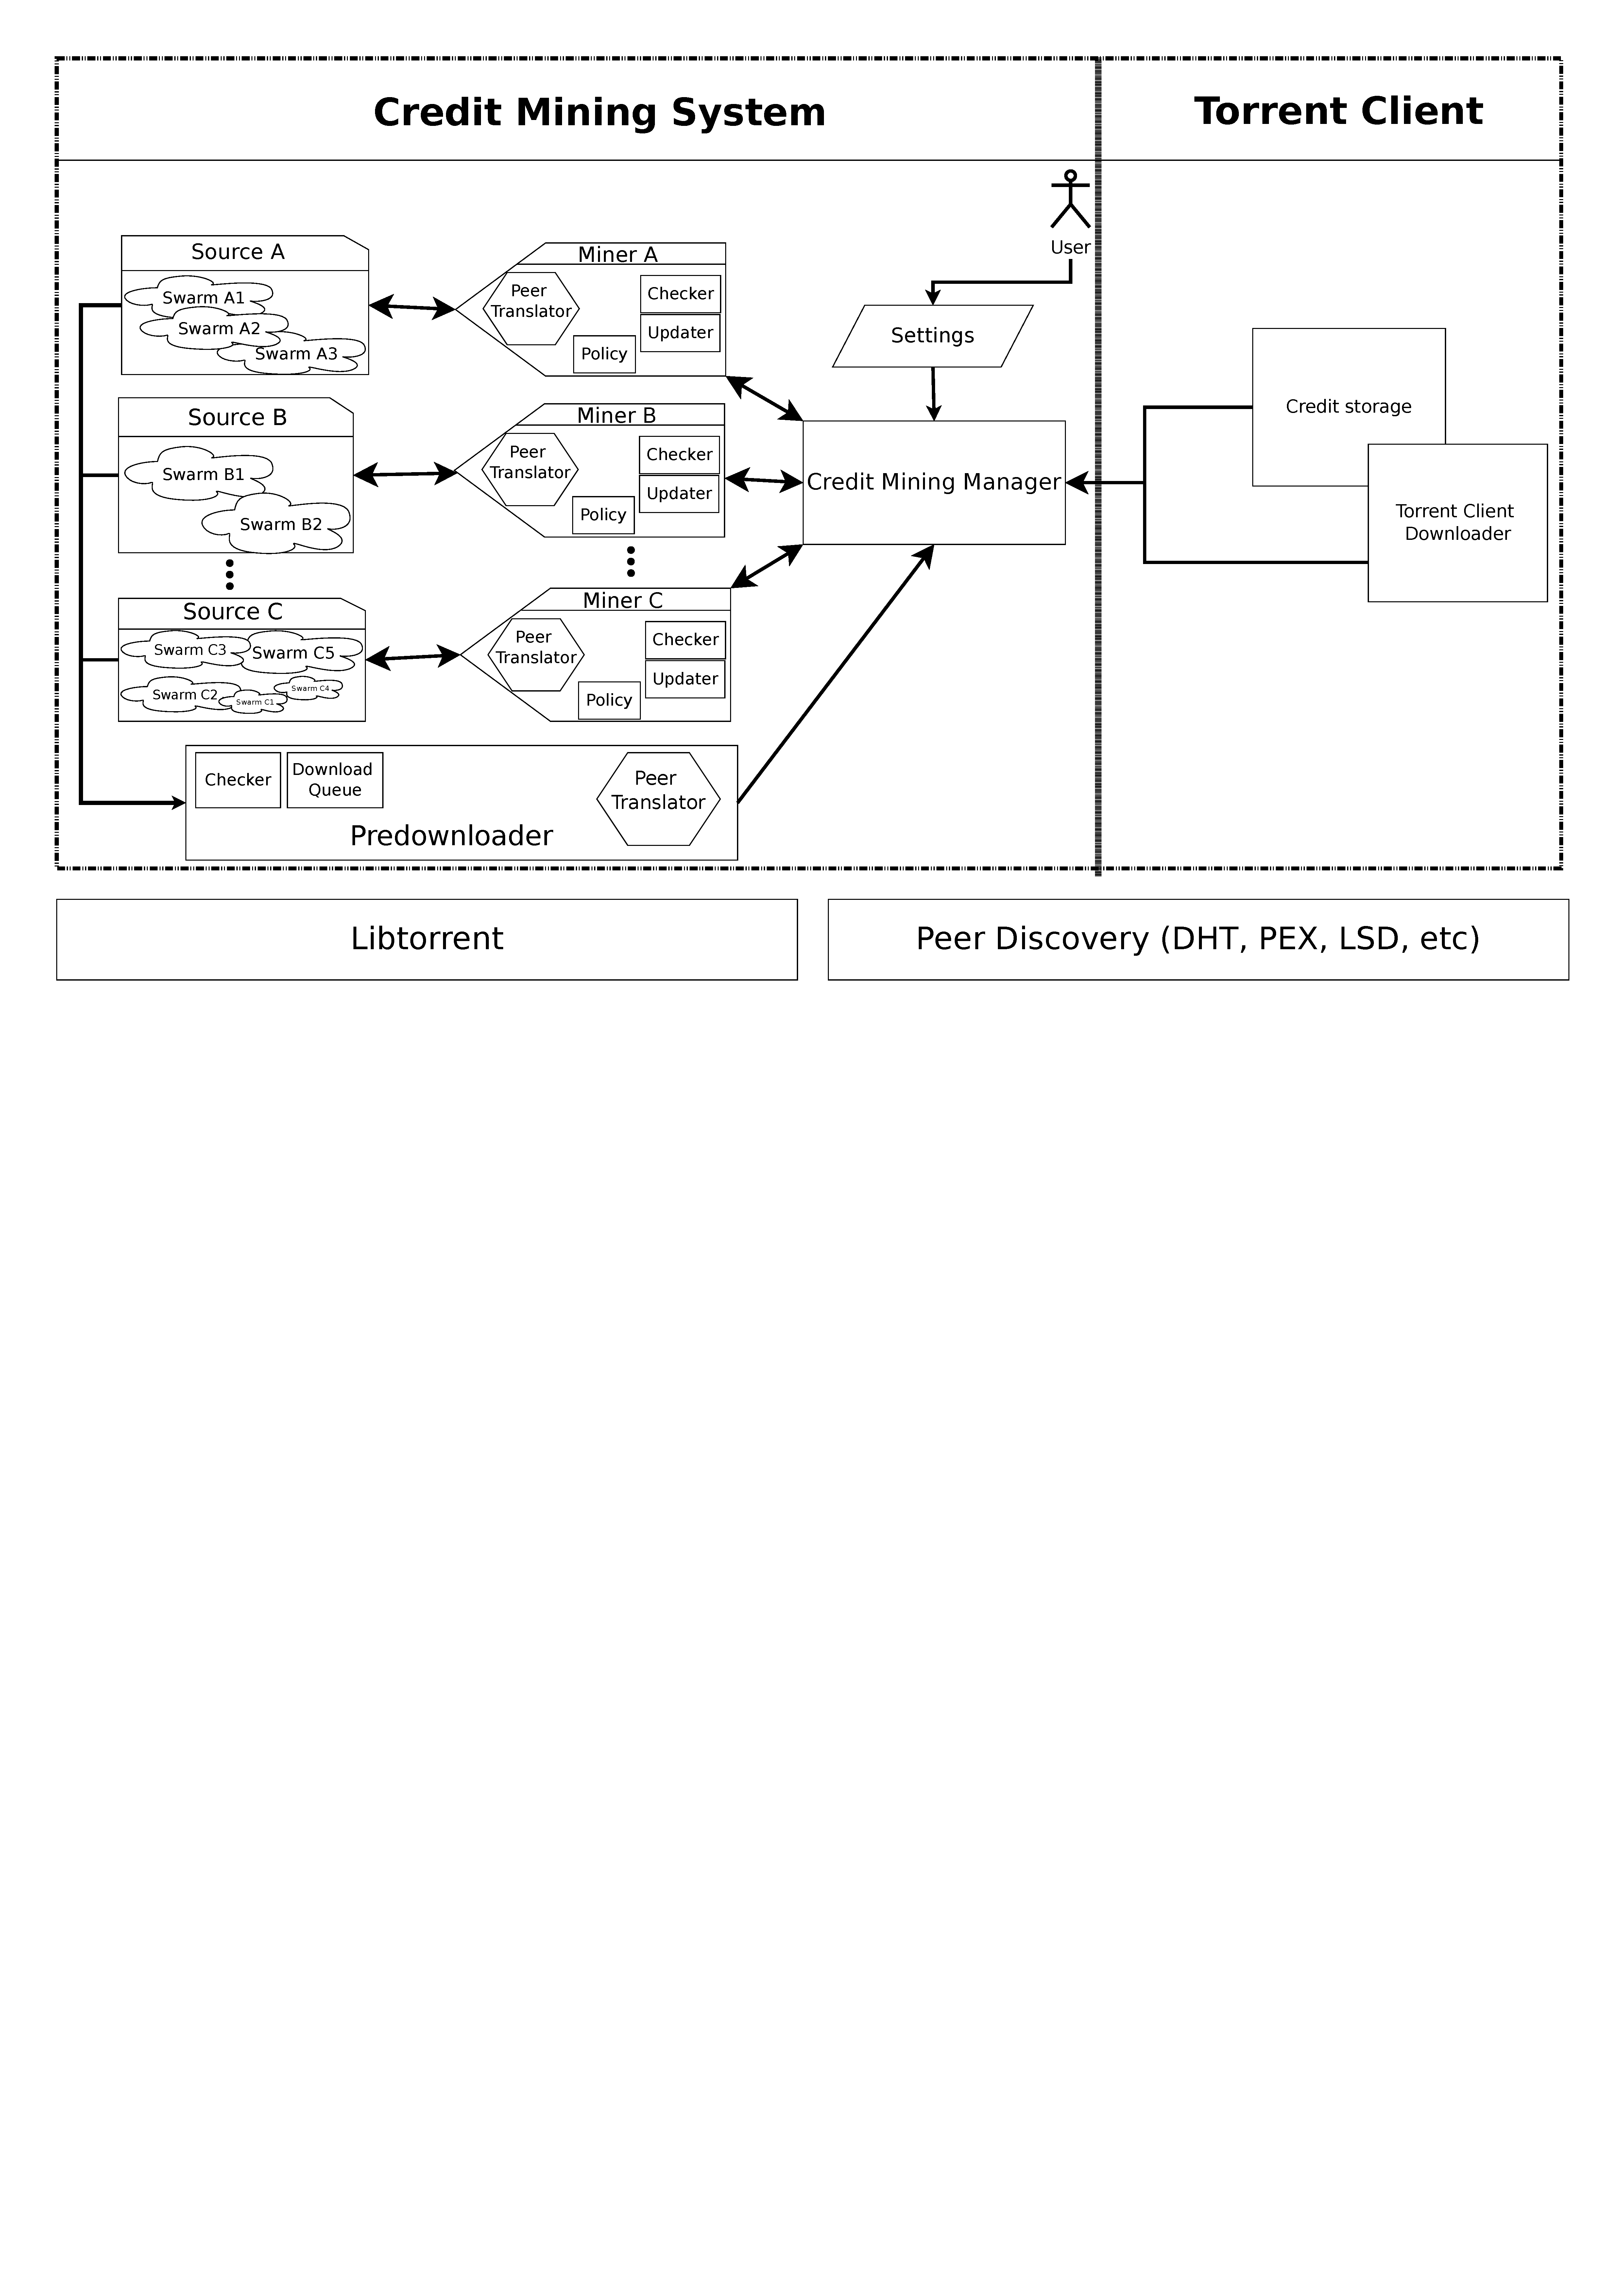
\includegraphics[width=\textwidth]{pics/cm_components.pdf}
	\caption{Credit mining components.}
	\label{fig:cmcomponents}
\end{figure}

% general flow
First, user can change the default settings used in the credit mining system. Some can not be changed when mining process run already. Table \ref{tbl:cmsettings} shows the settings used in this system. After user provide the setting and run the \textit{credit manager}, user can start mining by adding sources. A source usually consists of several swarms with different size, availability, and capacity. Each of the swarm will be assigned with one \textit{miner} that may have different type depends on the swarm itself. Before the miners start mining, \textit{predownloader} try to fetch swarm information as much as possible then give the results to the manager. Manager will propagate the swarm information to miners and let the miners decide which swarm to mine based on that information. Manager also monitor the main torrent downloader to adjust swarm's priority in miners. The credit gained from each of the miner will be reported to manager, then it forwards the results to credit storage in torrent client if necessary.

\begin{table}[h]
	\centering
	\caption{Credit mining settings}
	\label{tbl:cmsettings}
	\begin{adjustwidth}{-1.5cm}{}
	\begin{tabular}{|p{1cm}|p{4cm}|p{7cm}|p{2cm}|}
		\hline
		\rowcolor[HTML]{EFEFEF} 
		No. & Name & Description & Changeable at runtime \\ \hline
	1 & \textit{max\_torrents\_active} & The maximum number of simultaneous swarm that will be downloaded & Yes \\ \hline
	2 & \textit{max\_torrents\_per\_source} & The maximum number of stored torrent in a miner that will be considered for mining & Yes \\ \hline
	3 & \textit{source\_interval} & The interval needed to check for updates in the swarm & Yes \\ \hline
	4 & \textit{swarm\_interval} & The interval to re-evaluate swarm and start/stop swarm & Yes \\ \hline
	5 & \textit{share\_mode\_target} & Libtorrent share mode target (See Section \ref{section:sharemode}) & No \\ \hline
	6 & \textit{policy} & The policy used in mining (See Chapter \ref{chapter:prospection}) & No \\ \hline
	7 & \textit{logging\_interval} & The interval for logging, for debugging purpose & No \\ \hline
	8 & \textit{tracker\_interval} & The interval to check for a new peer by peer discovery methods & No \\ \hline
	9 & \textit{timeout\_torrent\_activity} & The maximum time threshold to mark a swarm as 'inactive' & Yes \\ \hline
	10 & \textit{piece\_download} & The number of piece what will be downloaded in \textit{predownload} phase & No \\ \hline
	\end{tabular}
	\end{adjustwidth}
\end{table}

Credit mining system is designed to be highly customizable. Some of the components can be extended or replaced. For example, the policy used to select the swarm. Beside what we proposed, user can define the policy as long as it overrides a function that return which swarm to start and stop. For peer translating, it is possible to override the function considering peer list and its information as an input, while returning number of seeder and leecher. Some value in the settings can be adjusted to match user's need and resource. With higher memory available, it is desirable to mine many swarms in one time by changing \textit{max\_torrents\_active} parameter. By having large storage, increasing \textit{piece\_download} may result a better return.

%The rest of this section will discuss key points of credit mining system. Several mining source types are supported with different treatment from miners. Prospecting methodology on top of libtorrent share mode will be elaborated afterwards. The methodology consists of two integral stages. Each of the stage has their own mechanism and requirements. Lastly, we will discuss other components that can support credit mining system of its prospecting, performance, and credit gain. 

\subsection{Mining Sources}
\label{section:msource} 
Currently, credit mining can accommodate three types of sources. There are directory source, RSS source, and channel source. In credit mining system, one source is assigned to one miner. The miner will start working the moment the source is defined and added to the manager. A miner periodically perform checking and other operations on all the torrents in the source. The operation that run in specified interval implemented differently for each of the source type. 

First type of source which called \textit{directory source}, is very straightforward. It takes a path as an argument and verify it before run the miner. The miner starts by looking at all the file in specified directory that have \texttt{.torrent} file type. Each of the file is examined and validated. Corrupt or invalid file will be discarded and deleted automatically from the disk. To keep the performance and prevent disk bottleneck, the miner sort the files alphabetically and put it into queue one by one. Miner periodically monitor both the directory if there is a new file and the queue to assign it to the manager. Miner eventually will pop an item from the queue, build a suitable format for mining, and notify manager to include this swarm.

Next possible mining source is from RSS (Rich Site Summary). RSS is a well known method to fetch new published data from a web. An RSS document contains the list of affected content which usually has summarized text and metadata. XML (Extensible Markup Language) format is widely used in RSS because of its compatibility and efficient size. An RSS from torrent portal such as etree\footnote{\url{http://bt.etree.org/rss/bt_etree_org.rdf}} and mininova\footnote{\url{http://www.mininova.org/rss.xml}} usually have title, publication date and a link to the swarm. Some mention number of seeder and leecher in the document. We called a source of RSS document as \textit{RSS feed}. 

In \textit{RSS source}, we assume that the RSS link user provided is available. If by any case the retrieval of the content is failed, the miner will stop immediately, notify the manager to disable this source, and shutting down itself. If the initial content retrieval is success, update mechanism will be launched periodically. In this mechanism, miner will fetch newest content from RSS feed. This content then parsed, resulting a list of swarm link and its metadata. Miner then asynchronously download the complete swarm data either via \texttt{.torrent} or magnet link. The same link will not be downloaded twice. After fetching the data, miner will build a defined format for mining, and notify manager to include this swarm. This data held across session. That means, another miner also will not download this swarm data in case it is indexed by other RSS feed.

\textit{Channel source} is the last type of source which tightly related to Tribler environment. As mentioned in section \ref{section:tribler} (Table \ref{tbl:community}), channel is responsible for managing torrents and playlists in Tribler community. A single channel can be discovered in \textit{AllChannel} community. Channel is identified by unique 40-length hexadecimal string. Naturally, Tribler user can create their own channel, put torrents into the channel, and share to other user. It is also possible for user to add a torrent to another user's channel. When a user subscribe to a channel, they will be notified if new torrent is added into that channel. Moreover, the torrents will be automatically downloaded into Tribler's database.

The flow of channel source is quite different with other type of source. It is tailored to follow Tribler specification which can change in the near future. Provided the identifier of a channel, miner will continuously try to find and join the channel in \textit{AllChannel}. By joined the channel, miner can get the list of torrents and other of its properties. After miner joined the channel, the swarm information will be handled and downloaded by Tribler. What miner do is to monitor the local database whether a new data has been fetched and there is a space for adding possible new torrent to the manager. Providing the swarm information, miner will download the \texttt{.torrent} file. It can be downloaded by using several options such as DHT, magnet link, or download from Tribler peers using TFTP (Trivial File Transfer Protocol). Downloaded \texttt{.torrent} will be stored in Tribler database. Afterwards, the mining format will be built and manager will be notified of a ready swarm.  

\subsection{Resource Optimization}
\label{section:optimization}
In this section, we focus on several optimizations that can be implemented in credit mining system. These optimizations are optional and can be left out. However, as the system itself is not without flaws, an improvement to support this system is advantageous. In general, there are two categories of support : helping get more credit in swarm and improving system resource utilization. The summary of designed optimizations are shown in Table \ref{tbl:optimizations}.

\begin{table}[t]
	\centering
	\caption{Credit mining optimizations}
	\label{tbl:optimizations}
	\begin{adjustwidth}{-1.5cm}{}
		\begin{tabular}{|p{0.7cm}|p{4cm}|p{10cm}|}
		\hline
		\rowcolor[HTML]{EFEFEF} 
		\hline
		\textbf{No} & \textbf{Optimization}& \textbf{Short Description} \\ \hline
		1  & Eliminate duplicates  & Removing identical files in swarm to mine \\ \hline
		2  & Swarm blacklisting    & Avoid picking slow swarm that has been previously invested\\ \hline
		3  & Inciting Swarm & Optimistically download new rarest piece if it idle too long\\ \hline
		4  & Starvation prevention & Immediately stop a swarm that idle for a long time and replace it with another one\\ \hline
		5  & Fallback mechanism    & Always pick \textit{default policy} whenever no swarm started although there are slots available \\ \hline
		6  & Reusing cache         & Reusing downloaded content when restarting the swarm instead start from nothing \\ \hline
		\end{tabular}
	\end{adjustwidth}
\end{table}

\subsubsection{Economic gain support}
In preliminary work by \citeauthor{2015:creditmining:capota}, credit mining system able to distinguish duplicate content in the P2P communities. It is highly possible that an exact same file have different infohash. An infohash of a torrent can come from many aspects such as different piece size, categorized as private or public swarm, or even directory name of the files \cite{2015:creditmining:capota}. We used \textit{Levenshtein distance} to measure the different between one swarm and another by considering the files and its length. In the end, we only mine the one who has higher number of seeder. The swarm comparison executed whenever there are new swarm reported by the miners. By eliminating duplicates in P2P communities, the supply and demand of a particular file can be focused. By focusing supply and demand into few swarms, the performance of participating peer might be improved \todo{Exclude archive mode in mihai's work because the implementation is not clear}.

In prospecting, it is possible that not all the swarm prospected can have good results. Regardless of the policy used, every miners will try to find best swarm in their library. In \textit{scoring policy} for example, miner will always try to mine best swarm found although it has very low score. In \textit{seeder ratio policy}, as long as there are peers in the swarm, a swarm will have a chance to be mined. On one hand, it is difficult to measure a swarm without joining it first, that is by downloading and seeding in that swarm. On the contrary, optimistically mine swarm may lead to sub-optimal performance. We argue that this is not necessarily a bad thing. By \textit{swarm blacklisting}, low performance swarm can be flagged and avoided in a longer term. Miner periodically check the performance of its swarm. \textit{Swarm blacklisting} also run in that period. Miner watch the when a particular active downloading or uploading data. If no activity detected in a swarm in a long period of time, the miner will remove this swarm from its library, Note that the swarm has a chance to be added to library again after several rounds. Moreover, blacklisted swarm can also be recovered if the performance of the rest of the swarms are not better and it has fulfill its threshold time. 

\subsubsection{Improving performance}
Credit mining system is designed to be deployed in end-user machine. With limited resource, it is a necessity to prevent resource waste as much as possible. We proposed following mechanism to improving the performance and use the resource as efficient as possible. 

Not all the swarm predicted by credit mining system is a good source. If a source itself only contains oversupplied swarm, the system will still optimistically mine something from it. Although switching to other swarm will eventually happen in purpose of equally distribute the credit, it will take quite a bit of time. \textit{Starvation prevention} will detect the swarm which does not have any activity in a period of time, then it will terminate that swarm immediately. Also, if the swarm is inactive for the majority of the period, it will also be terminated in end of the round. That is, by removing that swarm data in the cache and local memory to free some spaces for mining other swarm. Moreover, blacklisting swarm comes after this function. A swarm that has been terminated by this function is blacklisted as well. So it will not get any mining allocation in the next several turns.

% not include fallback (it doesn't make sense anymore)
As part of the prospecting process described in \ref{chapter:prospection}, miners select a swarm by its \textit{swarm selection} policy. However, depends on the circumstances, the result of this selection process may negate the result of previous round. In a case where the data used in policy changed, as caused by multiple tracker or incomplete information, negating one after another will harm the mining process. We want to avoid this issue by not permitting a swarm to be started in the following round when it was stopped. Likely, if the swarm is not suffer from starvation and not blacklisted, although the speed is low, it will not stopped in the following exact round after it was started. Because of this, credit mining system assures that a swarm at least run within two period. The idea is to give a second chance to low-performing mining if and only if there are no better swarm available.  The resource then can be fully utilized in response of the collection of unhealthy swarm. \todo{note: removed fallback}

Credit mining system is not intended to download a whole file completely. In this sense, there is a high probability that downloaded files will never complete. In the prior work, it is important to notice that after mining for a certain swarm was stopped, miners will delete downloaded files to save the storage. Although it is safe for the system to discard downloaded files, the resource used to redownload piece will be costly. This aspect is improved in the credit mining system. Files from a swarm that has been stopped for mining is archived with its history and stored in cache. The history consists of the index of the piece that have been downloaded, peer information, statistics, and many others. The downloaded files usually contains many padding piece, whose size can be significantly reduced from archiving. Dearchiving process may take time, but in return, credit mining system can continue mining from where it left. Moreover, if there are new peers requesting piece the system already have, it can be immediately uploaded.